\section{FPGA}

\subsection{PWM Driver}

PWM driveren har til opgave at levere et PWM-signal, med en duty cycle bestemt af et input fra microcontrolleren. Denne sektion vil beskrive designet af driveren samt nogle af de bevæggrunde der har ligget bag valget af dette design.

\subsubsection{Designmål}

\begin{itemize}

\item PWM frekvens mellem 20 kHz og 25 kHz
\item 8 bits PWM opløsning
\item Inputtet skal latches før duty cycle ændres

\end{itemize}

\subsubsection{Inputs}

Hovedårsagen til at der bliver brugt et 8 bits input til at vælge duty cycle, er at denne størrelse tit bliver brugt i microcontrollere, da arkitekturen er bygget op omkring data i forskellige byte-størrelser. Denne begrænsning findes som sådan ikke på en FPGA, da man selv kan lave sin arkitektur som man vil. Men hvis man formindsker bitstørrelsen for effektivitetens skyld, formindsker man også opløsningen for den duty cycle man kan vælge, og det er måske ikke hensigtsmæssigt i et kontrolsystem. Som udgangspunkt virker en opløsning på 8 bit som et fint kompromis XXXX.

Driveren har også brug for et clock-signal til at regulere timingen i den samt et latching input. Dette input lader PWM-modulet læse værdien af input-bus'en ind i driveren's egen hukommelse og derved ændre duty cycle.

\subsubsection{PWM Frekvens}

Der er en række ting man skal være opmærksom på, når man vælger frekvensen pulserne skal sendes ved. Jo højere frekvensen er, jo mere tid tilbringer man i switching transistoren's aktive område - det vil sammenlagt give et større effekttab. Frekvensen er til gengæld også nødt til at være høj nok til at motoren's inerti kan bløde de elektriske pulser ud rent mekanisk. Derudover er det også nemmere for motorspolerne at holde strømmen nogenlunde konstant ved en højere frekvens - det er blandt andet en af antagelserne fra den matematiske motormodel. Der skal også tages højde for de vibrationer, der genereres når motorinputtet kommer i pulser. Hvis frekvensen er mindre end 20 kHz, ligger vibrationerne inden for det hørbare område for mennesker, og det er ikke altid hensigtsmæssigt. Motoren og ophængets egenfrekvens skal også undgås - denne frekvens vil være højere jo mere stift ophæng motoren har, men den vil typisk ikke ligge i det supersoniske område. Alle disse ting peger tilsammen imod en PWM frekvens på den anden side af 20 kHz, men ikke meget derover. 

Med et 8 bits input skal hver pulsperiode deles ind i 256 lige store dele, så det er muligt at flytte tidspunktet, hvor der skiftes fra høj til lav og dermed få en anden duty cycle. 

\begin{equation}
T_{PWM}=\dfrac{1}{25 kHz} = 40 \mu s
\end{equation}

\begin{equation}
T_{slice}=\dfrac{T_{PWM}}{256}=156ns
\end{equation}

En clock-periode med FPGA'ens krystal på 50 MHz er $20ns$ lang, så hvis man tæller en variabel op hver 8. clock-periode til den når 256, så får man en samlet periodetid på $20ns*8*256=40.96 \mu s=24.414kHz$. Denne variabel sammenlignes så med den lagrede 8 bits duty cycle værdi, for at afgøre om signalet på udgangen skal være højt eller lavt.

\begin{figure}[h]
	\begin{center}
		\includegraphics[scale=0.5]{Billeder/PWM_Timing.png}
	\end{center}
\label{fig:PWM_timing}
\caption{Ramperne på den øverste graf repræsenterer variablen der tælles op fra 0 til 255. På den nederste graf ses det resulterende PWM-signal}
\end{figure}

\subsubsection{Positions modul}

For at kunne ramme et punkt på himlen, bliver microcontrolleren nødt til at vide hvilken position pan-tilt systemet står i.
For at kende denne position, er der to hall sensorer på EMG30 motoren.
Disse sensorer sidder 90 grader forskudt, når motoren har kørt en omgang (Den indre rotor) har hall sensorerne sendt høj 3 gange hver.
Hver gang en hall sensor går fra høj til lav, eller lav til høj, vil et register i FPGA'en inkrementere et register med 1.\\

For at kunne finde ud af hvilken vej motoren kører, kigges der på hvordan hall sensorerne går høj og lav i forhold til hinanden.

\begin{figure}[h]
	\begin{center}
		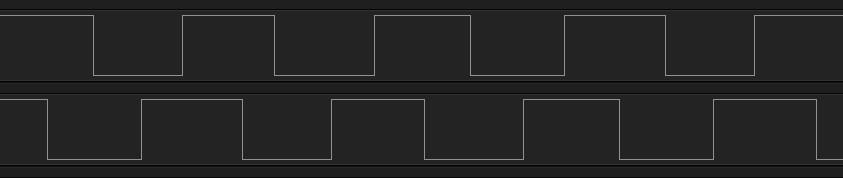
\includegraphics[scale=0.5]{Billeder/Hall_sensorer.png}
	\end{center}
\label{fig:Hall_Sensorer}
\caption{Her ses et billede af hvordan hall sensorerne går høj og lav i forhold til hinanden}
\end{figure}

Rotation.
Når hall sensor 1 er høj, og hall sensor 2 er høj\\
Hvis så hall sensor 2 bliver lav først, så er det en rotation med uret.\\
Og hvis hall sensor 1 bliver lav først, så er det mod uret.\\

Når hall sensor 1 er lav, og hall sensor 2 er lav\\
Hvis hall sensor 2 så bliver høj først, så er det en rotation med uret.\\
Hvis hall sensor 1 bliver høj først, så er det en rotation mod uret.\\